\newpage
\section{Progettazione}

\subsection{Progettazione Architetturale}

\subsubsection{Requisiti non funzionali}

Dall'analisi dei requisiti sono emersi i seguenti requisiti non funzionali:
\begin{itemize}
\item Tempo di risposta
\item Usabilità
\item Integrità dei dati
\item Protezione dei dati 
\item Sicurezza delle comunicazioni
\end{itemize}
La protezione dei dati e delle comunicazioni assume fondamentale importanza vista la natura del software, 
che deve trattare dati personali e sanitari dei clienti. 
La compromissione di questi risulterebbe in una grave perdita finanziaria e di immagine, senza considerare i danni apportati alla privacy degli utenti. 
Inoltre, sarà necessario assicurare la sicurezza fisica dei dati immagazzinati nel sistema.
L'introduzione di misure di sicurezza delle comunicazioni e protezione dei dati non compromette l'usabilità del sistema, ma potrebbe peggiorarne leggerlmente le prestazioni: 
è possibile comunque bilanciare le due esigenze senza eccessive complicazioni mediante le tecnologie esposte in seguito. 
Va notato inoltre che il sistema non presenta vincoli di tempo particolarmente stringenti (nessun vincolo real-time).

\subsubsection{Scelte tecnologiche}

La scelta tecnologica principale ricade sul tipo di applicazione che si andrà a sviluppare.
In questo caso la scelta è stata quella di sviluppare un'applicazione web, per vari motivi:
prima di tutto, consente di avere una piattaforma standard accessibile da quasi tutti i dispositivi,
con il solo requisito di un browser web. In questo modo si evita di restringere le possibilità di accesso al servizio.
Inoltre, un'applicazione web consente di avere una gestione maggiormente centralizzata ed un deployment più agevole (a questo proposito si veda la sezione apposita del deployment).


\subsubsection{Scelta dell'architettura}

Dopo una rapida analisi, si è constatato che l'architettura più adeguata per il sistema è l'\textbf{architettura client-server a 3 livelli}.

\paragraph{L1 -- Client}\mbox{}\\
La componente lato Client sarà implementata da due interfacce differenti:

\begin{itemize}
\item[-] Un'interfaccia per le funzionalità relative ai clienti (registrati e non)
\item[-] Un'interfaccia per la gestione della farmacia da parte di un operatore (farmacista)
\end{itemize}

\paragraph{L2 -- Server}\mbox{}\\
Rispettando il principio del "minimo privilegio" per limitare i danni in caso di attacco e per distribuire meglio il carico, si è deciso di scomporre i server in base alle funzionalità offerte. Si hanno quindi tre server:

\begin{itemize}
\item[-] Un server che fornisce i servizi ai clienti registrati e non
\item[-] Un server che funge da pannello di controllo per i farmacisti
\item[-] Un server per le funzionalità di autenticazione
\end{itemize}

\paragraph{L3 -- Persistenza}\mbox{}\\
La gestione della persistenza verrà implementata in un server dedicato sul quale sarà installato un DBMS che gestisca i dati di tutte le farmacie aderenti al servizio.
Su tale server sarà installato il DBMS IBM DB2.
L'interfacciamento con il DBMS avverrà mediante la metodologia "forza bruta" utilizzando i metodi CRUD.
Per quanto riguarda il log delle operazioni, invece, questo verrà salvato su file system (un semplice file sul server adibito)

\subsubsection{Pattern architetturali e di design}

Infine, dopo un'attenta analisi, si è optato per l'adozione del pattern \textbf{Broker}: 
un componente verrà interposto alla comunicazione Client--Server e avrà il compito di indirizzare le richieste dei client al relativo server, 
effettuando un controllo sulle sessioni attive per determinare lo stato del client. 
La scomposizione in diversi client e server consente di avere una separazione netta tra gli applicativi del cliente e del farmacista, 
in modo da localizzare le operazioni critiche e ottenere maggiore protezione dei dati.
Il pattern Model View Controller (\textbf{MVC}) è stato invece scelto come pattern architetturale.
\\
Chiaramente l'affidabilità del sistema dipende dalla robustezza del broker e soprattutto del sistema di autenticazione.
\\
Si riportano di seguito i diagrammi di package e componenti che descrivono l'architettura del sistema.

\newpage

\begin{figure}[h!]
    \begin{center}
        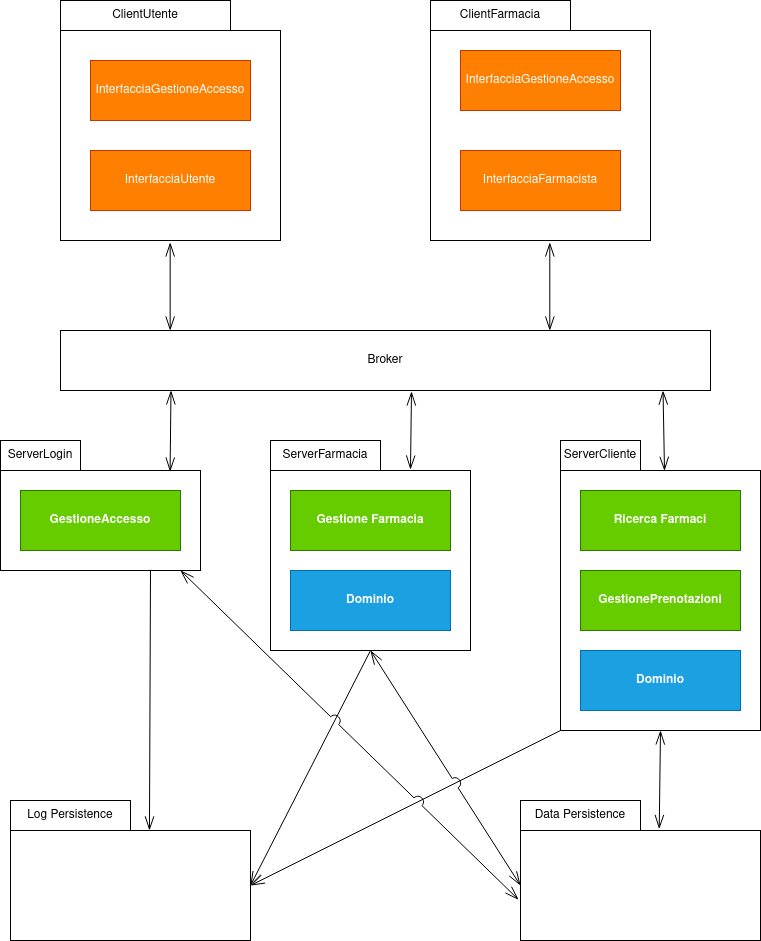
\includegraphics[width=\textwidth]{immagini/Package-progettazione.png}
        \caption{Diagramma dei package}
    \end{center}
\end{figure}

\newpage

\begin{figure}[h!]
    \begin{center}
        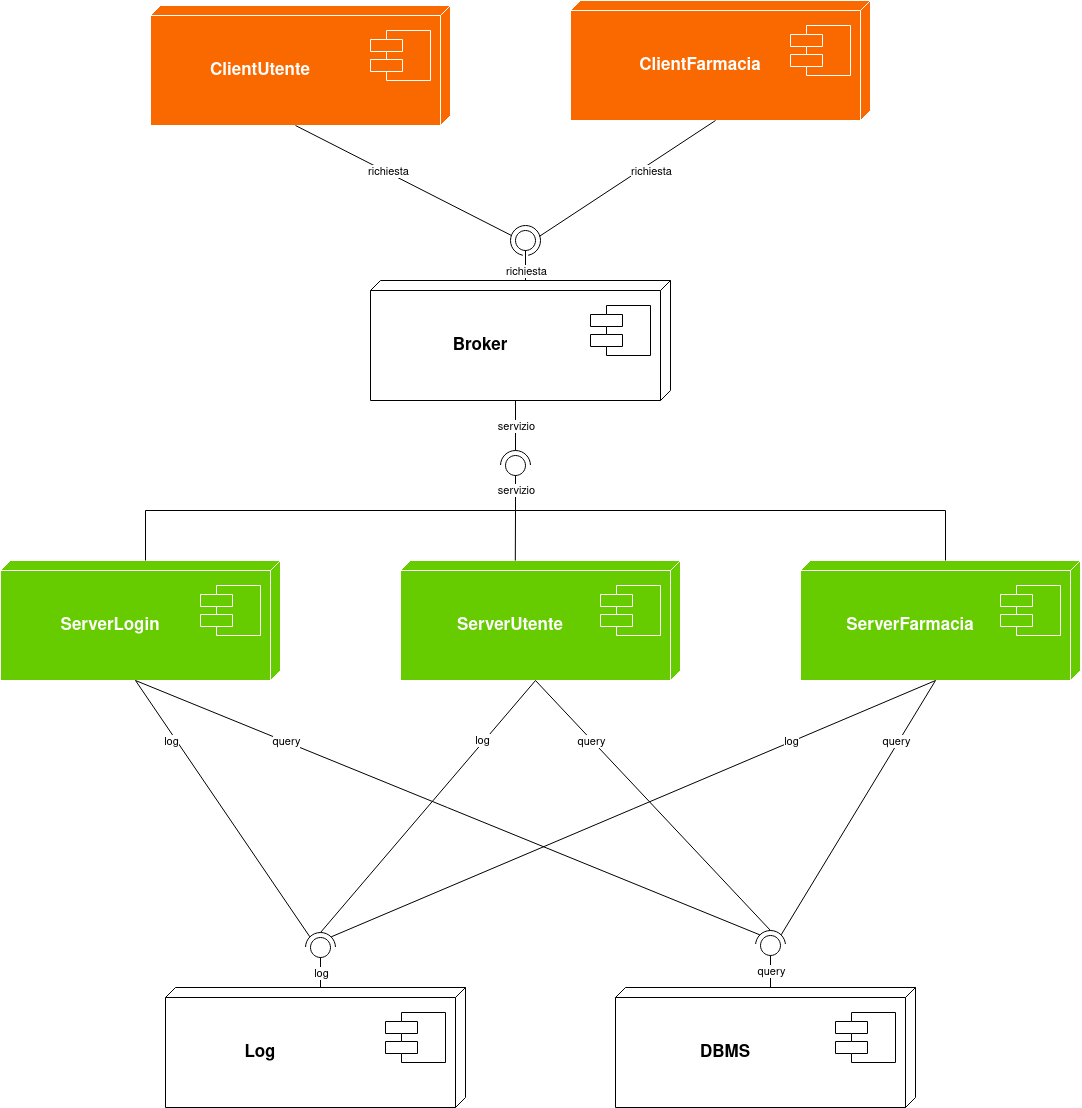
\includegraphics[width=\textwidth]{immagini/Componenti-progettazione.png}
        \caption{Diagramma dei componenti}
    \end{center}
\end{figure}

\newpage

\subsection{Progettazione di dettaglio}

\subsubsection{Struttura}

\textbf{Struttura: Dominio}\\

Per quanto riguarda il dominio, i diagrammi rimangono sostanzialmente uguali a quelli visti in analisi.
Nonostante il dominio del cliente sia pressoché identico a quello del farmacista, 
si è comunque deciso di distinguere i due domini al fine di evitare l'introduzione di classi non necessarie.
In particolare, la parte di applicativo relativa al cliente non dovrà gestire
né conoscere i farmacisti legati ad ogni farmacia (informazione nota solo al
server delle farmacie).

\vspace{2em}

\textbf{Diagramma di dettaglio: Dominio Clienti}

\begin{figure}[h!]
    \begin{center}
        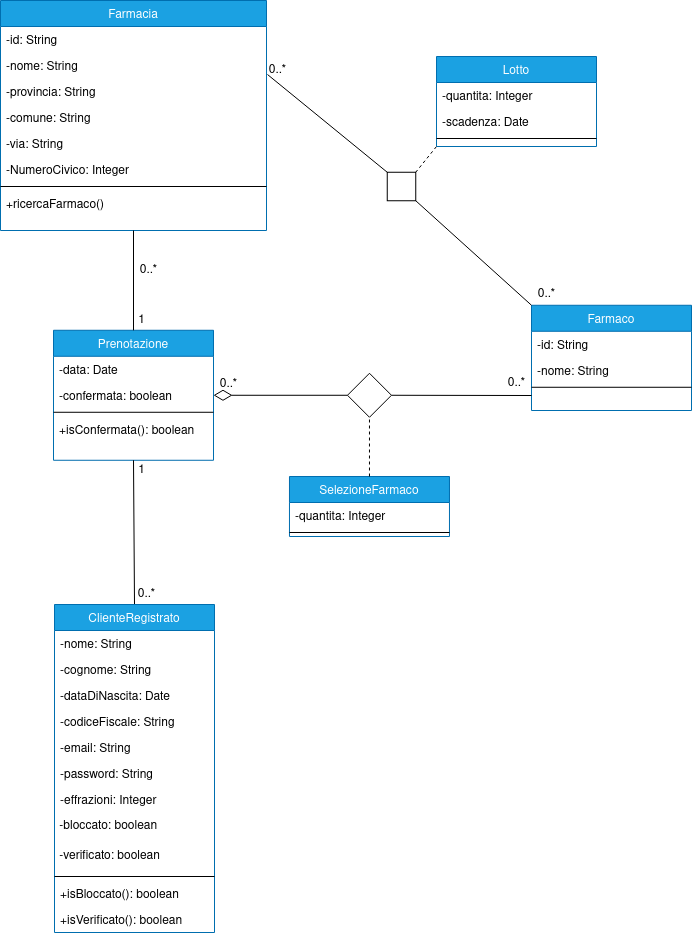
\includegraphics[scale=0.53]{immagini/DominioCliente-progettazione.png}
    \end{center}
\end{figure}

\newpage

\textbf{Diagramma di dettaglio: Dominio Farmacia}
\begin{figure}[h!]
    \begin{center}
        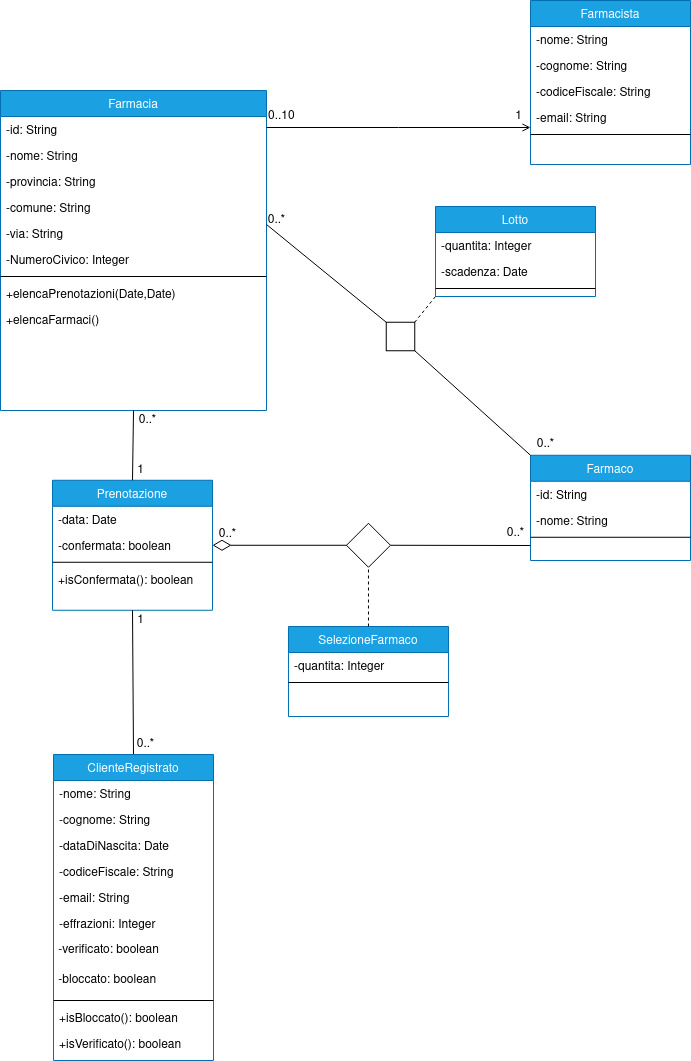
\includegraphics[scale=0.56]{immagini/DominioFarmacia-progettazione.jpg}
    \end{center}
\end{figure}

\newpage

Come si può notare, il dominio della farmacia presenta diversi metodi aggiuntivi (in particolare per effettuare operazioni sul cliente e per elencare farmaci)
non necessari al cliente e anzi da nascondere ad esso per evitare che i permessi o privilegi vengano aggirati.
Inoltre, le associazioni \texttt{Lotto} e \texttt{SelezioneFarmaco} sono state mantenute nei diagrammi per chiarezza. 
L'associazione \texttt{Lotto} dovrà necessariamente essere una classe a sé stante,
mentre l'associazione \texttt{SelezioneFarmaco} potrà essere concretizzata in classe o sostituita da un semplice Integer. Quest'ultima scelta è lasciata agli implementatori.
Le associazioni vere e proprie dovranno poi essere implementate mediante una \textbf{mappa}, ad esempio con un oggetto del tipo \mbox{\texttt{HashMap<Farmaco, Lotto>}}
\vspace{2em}

\textbf{Diagramma di dettaglio: Interfacce}
\begin{figure}[h!]
    \begin{center}
        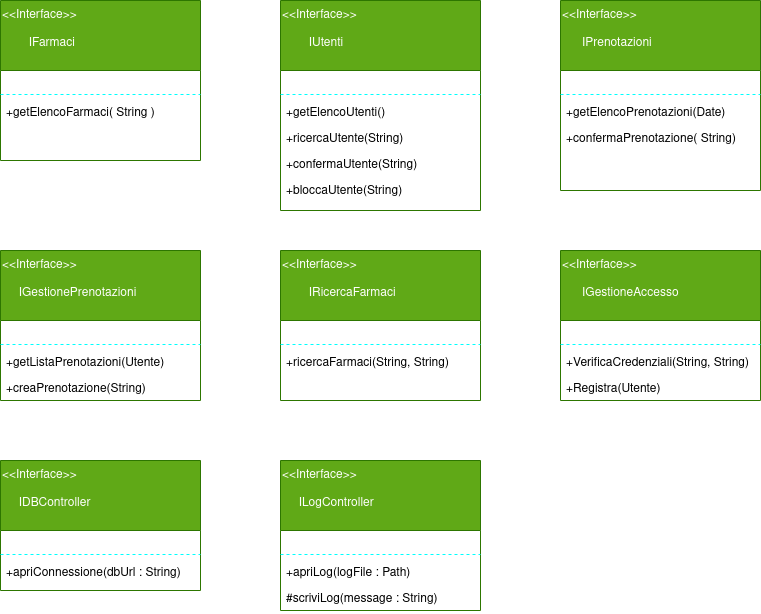
\includegraphics[width=\textwidth]{immagini/Interfacce-progettazione.png}
    \end{center}
\end{figure}

L'aggiunta di tali interfacce consente di applicare il \textit{Dependency Inversion Principle}
in modo da disaccoppiare gli utilizzatori dalle implementazioni, che potrebbero cambiare.
L'interfaccia \texttt{IMagazzinoObserver} è stata introdotta per l'utilizzo di un pattern Observer,
i cui dettagli vengono esposti nel prossimo paragrafo.

\newpage

\paragraph{Struttura: Controller}\mbox{}\\

Si è deciso di utilizzare una classe \texttt{Controller} in cui inserire le funzionalità relative alla persistenza (Database e Log).
Si è pensato di posizionare questa classe in cima alla gerarchia dei controller: 
in questo modo, le funzionalità comuni di lettura/scrittura su database e log sono riutilizzabili dai controller figli senza bisogno di reimplementarle.
Nonostante il controller "monolitico" non rispetti il \textit{Single Responsibility Principle}, 
abbiamo comunque optato per questa soluzione, in quanto le funzionalità relative al database e al logging risultano facilmente accoppiabili essendo entrambe legate a un qualche tipo di persistenza.
Inoltre, non si prevede alcun tipo di estensione/modifica per quanto riguarda la persistenza.
\vspace{2em}

\textbf{Diagramma di dettaglio: RicercaFarmaci, GestionePrenotazioni}
\begin{figure}[h!]
    \begin{center}
        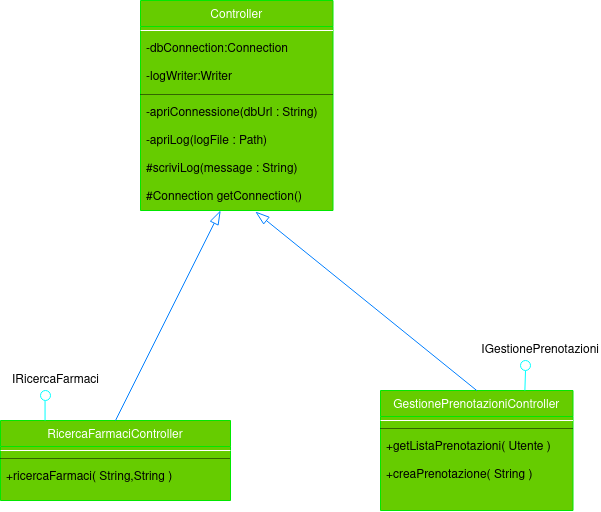
\includegraphics[width=\textwidth]{immagini/ControllerCliente-progettazione.png}
    \end{center}
\end{figure}

\newpage

\textbf{Diagramma di dettaglio: GestioneFarmacia}
\begin{figure}[h!]
    \begin{center}
        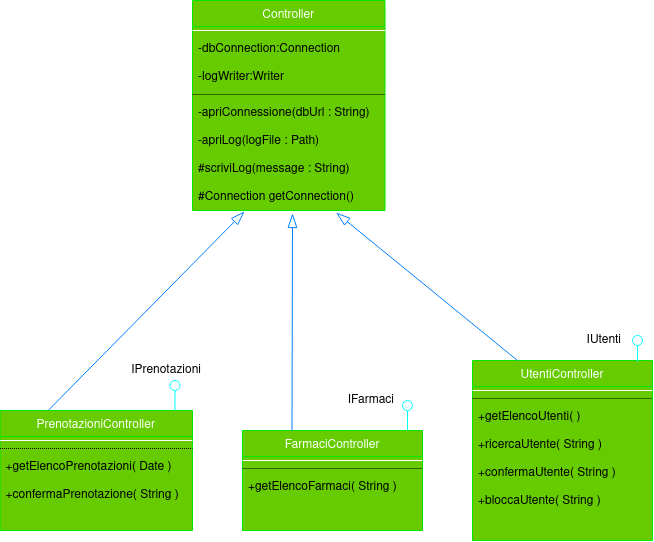
\includegraphics[width=\textwidth]{immagini/ControllerFarmacia-progettazione.png}
    \end{center}
\end{figure}

Anche i controller presenti sul server relativo alle farmacie seguono lo stesso principio esposto sopra.

\newpage

\textbf{Diagramma di dettaglio: GestioneAccesso}
\begin{figure}[h!]
    \begin{center}
        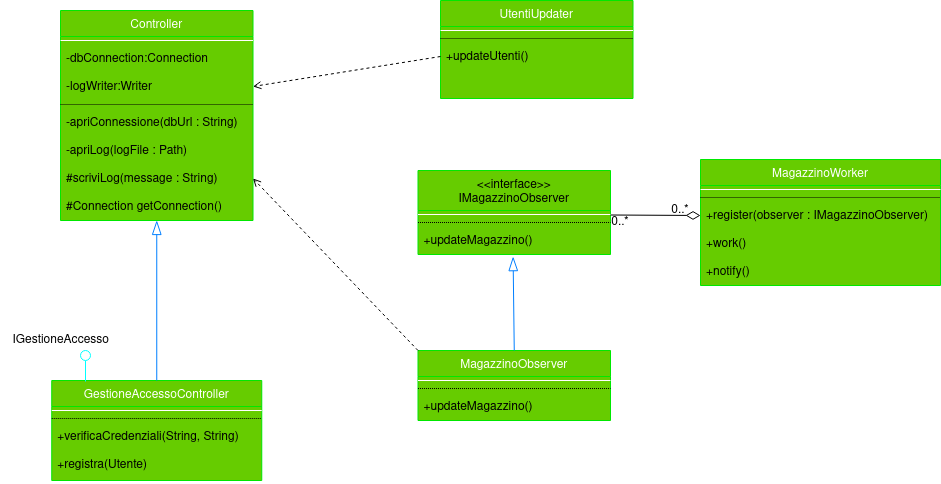
\includegraphics[width=\textwidth]{immagini/ControllerLogin-progettazione.png}
    \end{center}
\end{figure}

Il diagramma di dettaglio del server login risulta più complesso degli altri due
poiché contiene le ulteriori classi necessarie per implementare l'aggiornamento dello stato dei clienti
e caching del database in seguito al ricevimento di eventi.
In particolare, per implementare il caching locale del database remoto contenente i dati dei magazzini,
si è deciso di utilizzare un pattern \textit{Observer}: Un'istanza della classe \texttt{MagazzinoObserver} viene registrata
nel \texttt{MagazzinoWorker}. Quest'ultimo poi comunicherà con il server remoto mediante un protocollo prestabilito e,
alla ricezione di un aggiornamento da parte del server, notificherà l'Observer. Lo scambio dei dati riguardanti l'aggiornamento può avvenire tra Worker e Observer in diversi modi,
pertanto la scelta viene lasciata agli implementatori.

Si noti che la scelta del pattern Observer è dettata dal fatto che l'evento di aggiornamento del database remoto può risultare importante anche per future estensioni del software:
per questo motivo l'Observer si basa sull'interfaccia \texttt{IMagazzinoObserver}.

Per quanto riguarda invece l'aggiornamento dello stato dei clienti a fine giornata,
il metodo \texttt{updateUtenti()} della classe \texttt{UtentiUpdater} verrà invocato automaticamente
allo scattare di un nuovo giorno, in base all'orario del server.

\newpage

\textbf{Diagramma di dettaglio: Broker}
\begin{figure}[h!]
    \begin{center}
        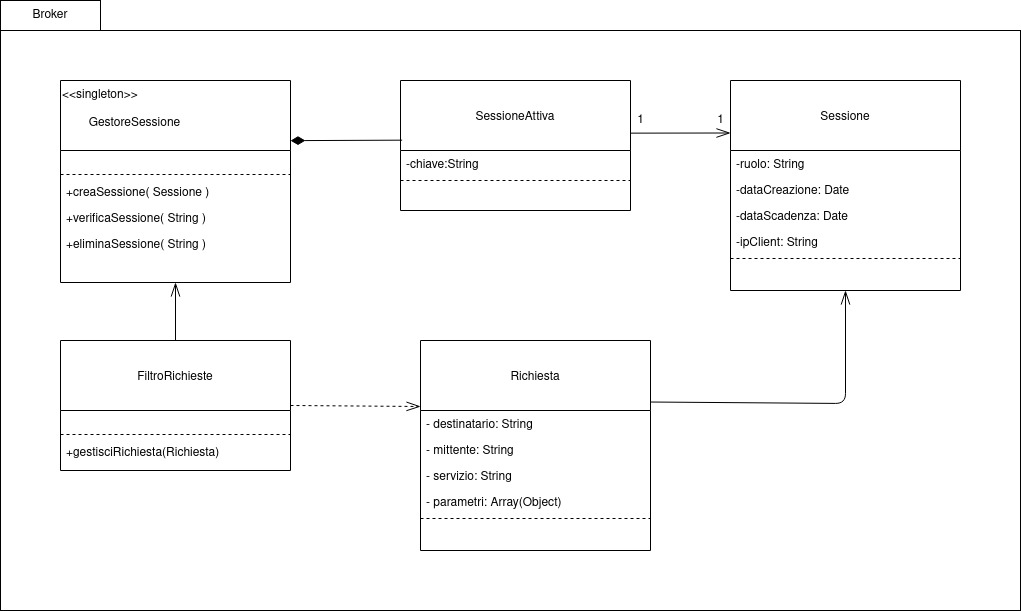
\includegraphics[width=\textwidth]{immagini/Broker.jpg}
    \end{center}
\end{figure}

\newpage


\textbf{Diagramma di dettaglio: InterfacciaUtente}
\begin{figure}[h!]
    \begin{center}
        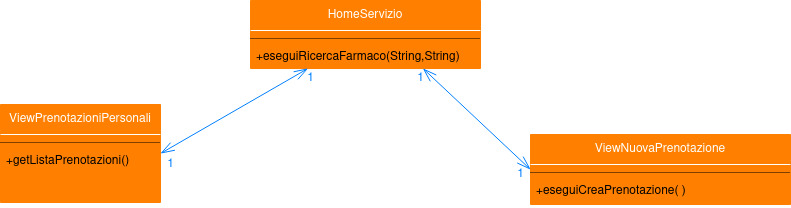
\includegraphics[width=0.9\textwidth]{immagini/ViewCliente-progettazione.jpg}
    \end{center}
\end{figure}

\begin{figure}[h!]
    \centering
    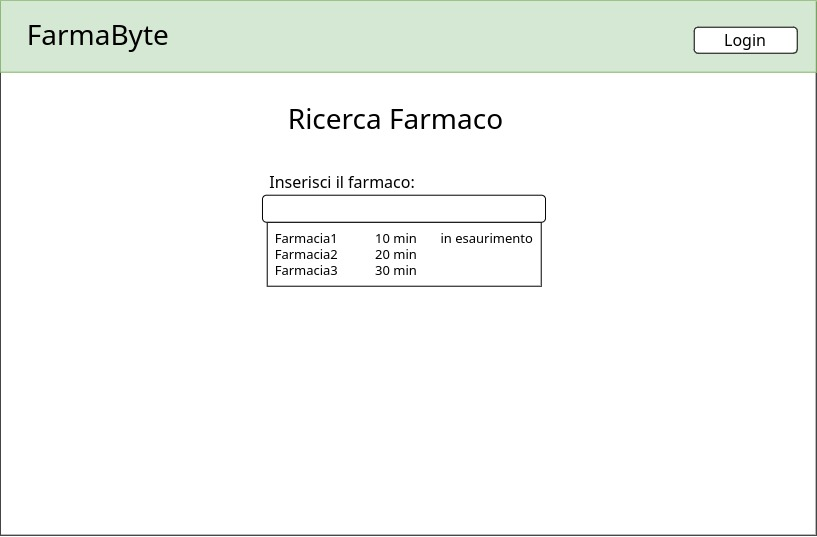
\includegraphics[width=0.9\textwidth]{VisteUtente-Home.jpg}
    \caption{Home}
\end{figure}
\newpage

\begin{figure}[h!]
    \centering
    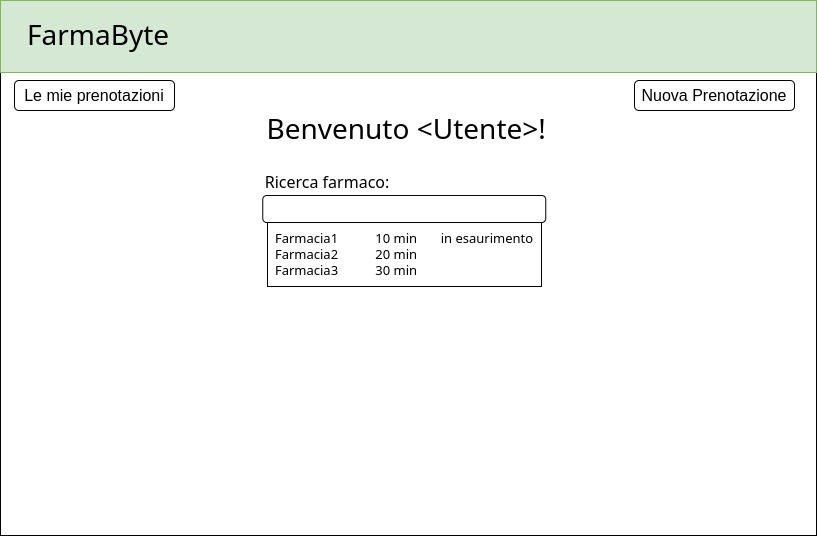
\includegraphics[width=0.9\textwidth]{VisteUtente-HomeLogin.jpg}
    \caption{HomeLogin}
\end{figure}

\begin{figure}[h!]
    \centering
    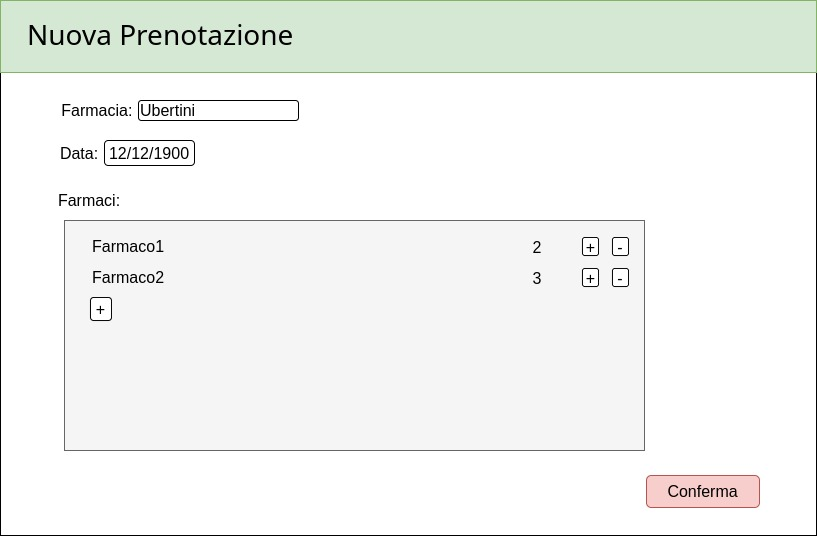
\includegraphics[width=0.9\textwidth]{VisteUtente-Nuova Prenotazione.jpg}
    \caption{Nuova Prenotazione}
\end{figure}
\newpage

\begin{figure}[h!]
    \centering
    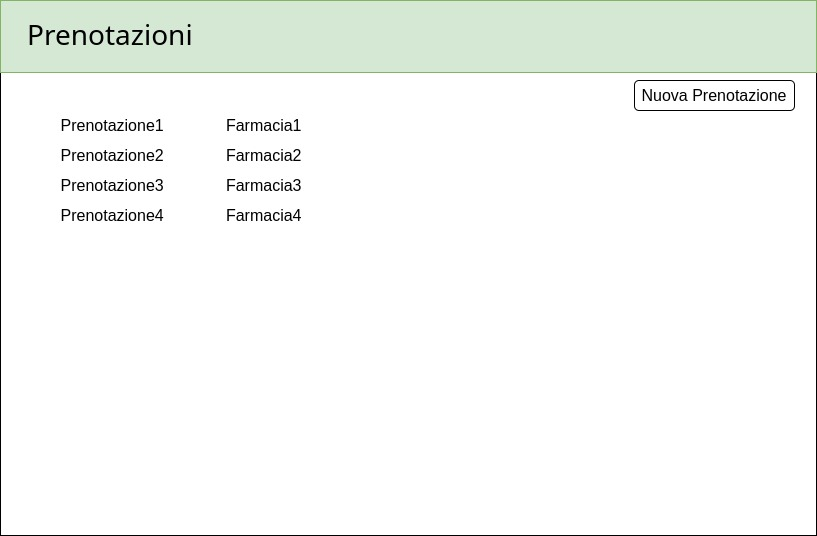
\includegraphics[width=0.9\textwidth]{VisteUtente-Prenotazioni.jpg}
    \caption{Prenotazioni}
\end{figure}

\newpage

\textbf{Diagramma di dettaglio: InterfacciaFarmacista}
\begin{figure}[h!]
    \begin{center}
        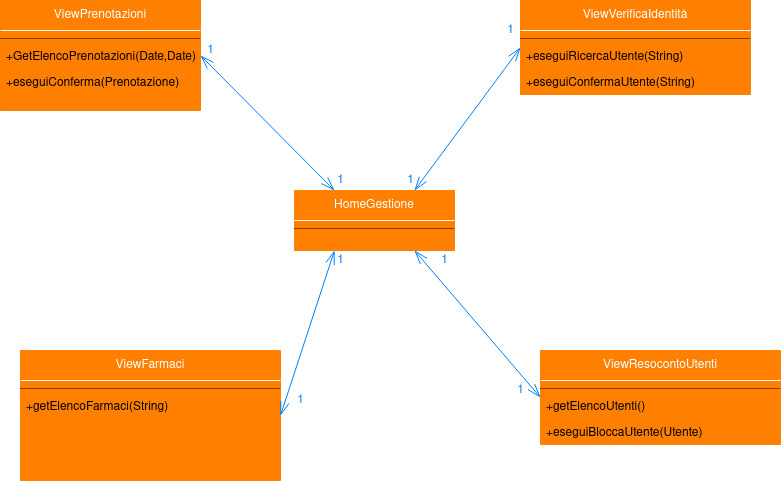
\includegraphics[width=0.9\textwidth]{ViewFarmacia-progettazione.jpg}
    \end{center}
\end{figure}

\begin{figure}[h!]
    \centering
    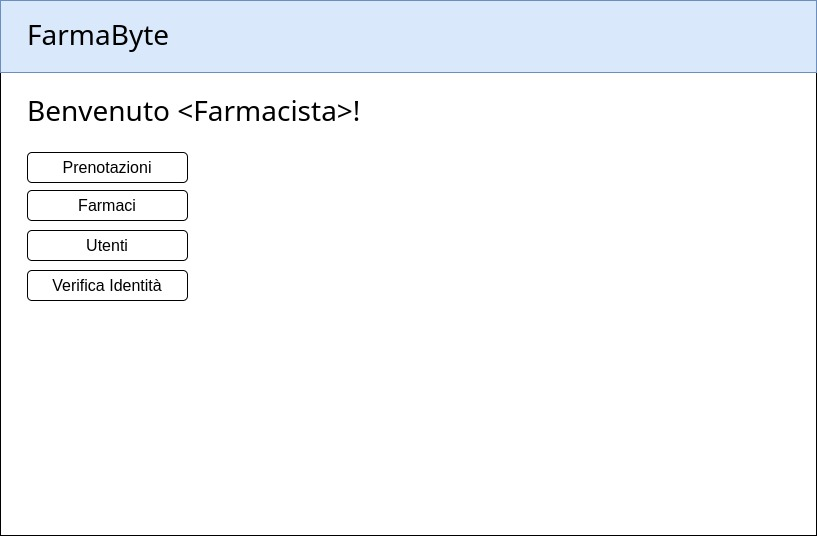
\includegraphics[width=0.9\textwidth]{VisteFarmacia-HomeFarmacista.jpg}
    \caption{Home}
\end{figure}
\newpage

\begin{figure}[h!]
    \centering
    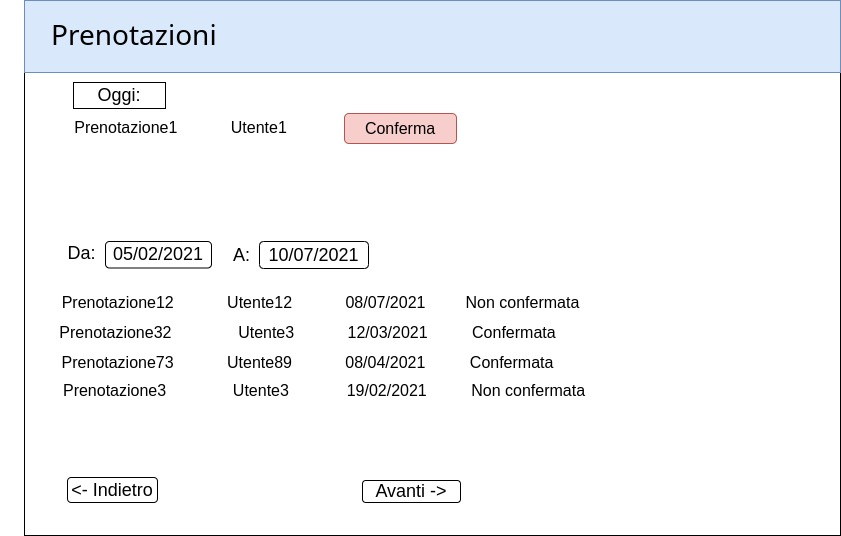
\includegraphics[width=0.9\textwidth]{VisteFarmacia-Prenotazioni.jpg}
    \caption{Prenotazioni}
\end{figure}

\begin{figure}[h!]
    \centering
    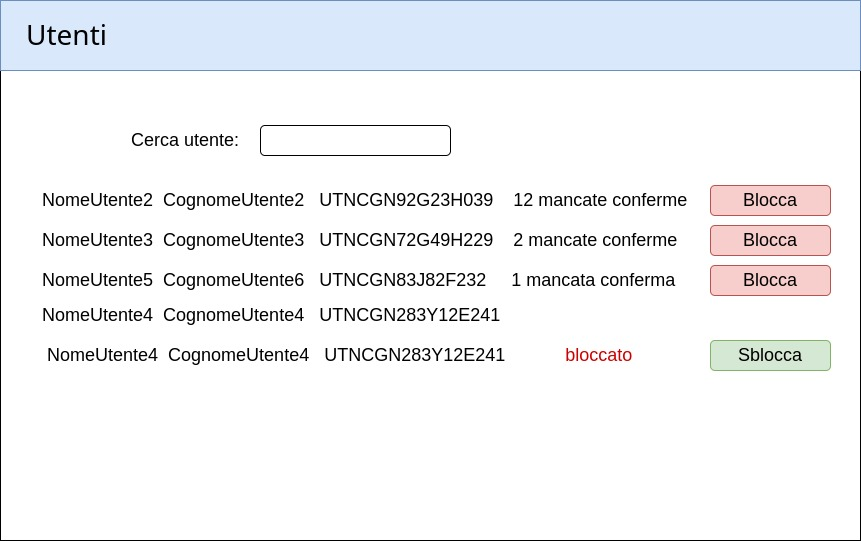
\includegraphics[width=0.9\textwidth]{VisteFarmacia-Utenti.jpg}
    \caption{Utenti}
\end{figure}
\newpage

\begin{figure}[h!]
    \centering
    \includegraphics[width=0.9\textwidth]{VisteFarmacia-Verifica Identità.jpg}
    \caption{VerificaIdentità}
\end{figure}

\vspace{3em}

\textbf{Diagramma di dettaglio: InterfacciaGestioneAccesso}
\begin{figure}[h!]
    \begin{center}
        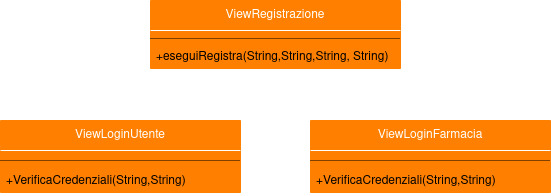
\includegraphics[width=\textwidth]{DettaglioBrokerLoginInterfacce-ViewLogin.jpg}
    \end{center}
\end{figure}

L'interfaccia di GestioneAccesso è composta dalle view che permettono a clienti e farmacisti di registrarsi e/o effettuare l'accesso al servizio.
Pertanto, è presente in entrambi i client, completata dalle ulteriori interfacce specifiche del client.
\\

\begin{figure}[h!]
    \centering
    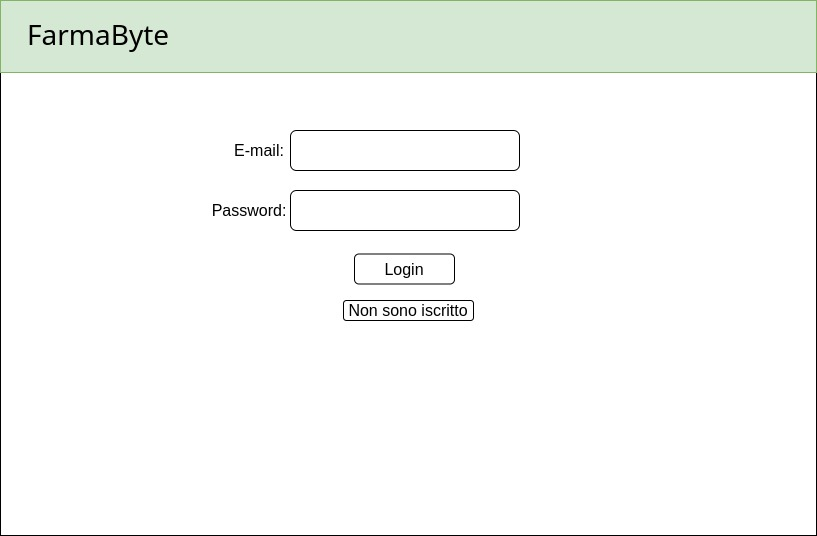
\includegraphics[width=0.9\textwidth]{VisteUtente-Login.jpg}
    \caption{Login Utente}
\end{figure}

\begin{figure}[h!]
    \centering
    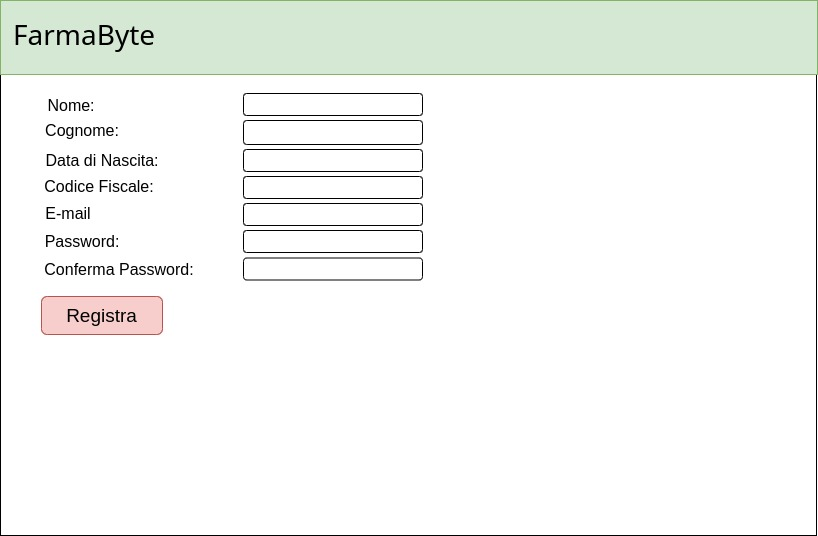
\includegraphics[width=0.9\textwidth]{VisteUtente-Registrazione.jpg}
    \caption{Registrazione Utente}
\end{figure}
\newpage

\begin{figure}[h!]
    \centering
    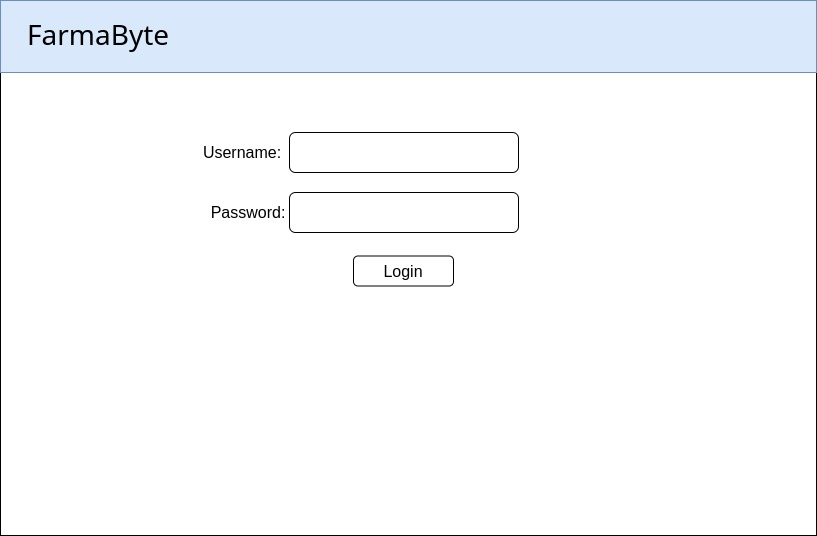
\includegraphics[width=0.9\textwidth]{VisteFarmacia-Login.jpg}
    \caption{Login Farmacista}
\end{figure}
\newpage

\subsubsection{Interazione}

Si riportano di seguito i vari diagrammi di sequenza, aggiornati rispetto a quelli visti in fase di analisi.

\vspace{3em}

\textbf{Diagramma di Sequenza: LoginFarmacista}

\begin{figure}[h!]
    \begin{center}
        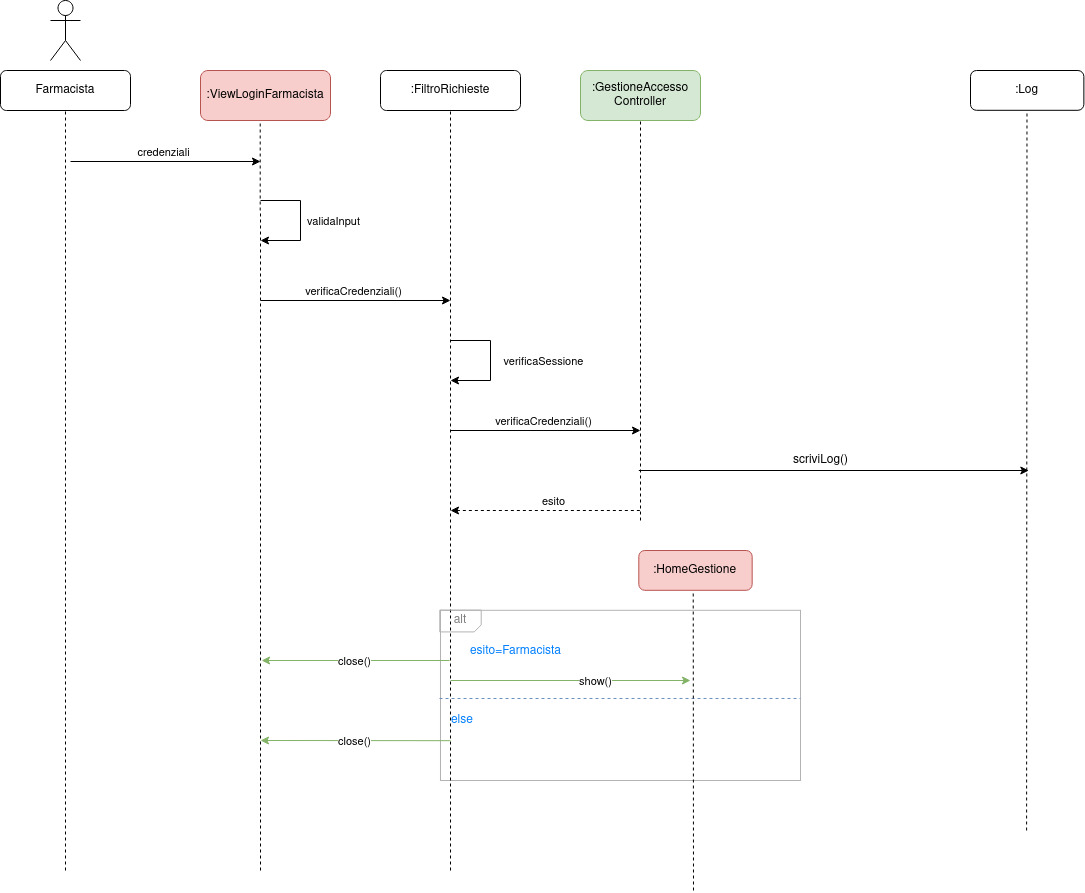
\includegraphics[width=\textwidth]{immagini/Interazione-LoginUtente-progettaz.jpg}
    \end{center}
\end{figure}

\newpage

\textbf{Diagramma di Sequenza: RegistrazioneUtente}

\begin{figure}[h!]
    \begin{center}
        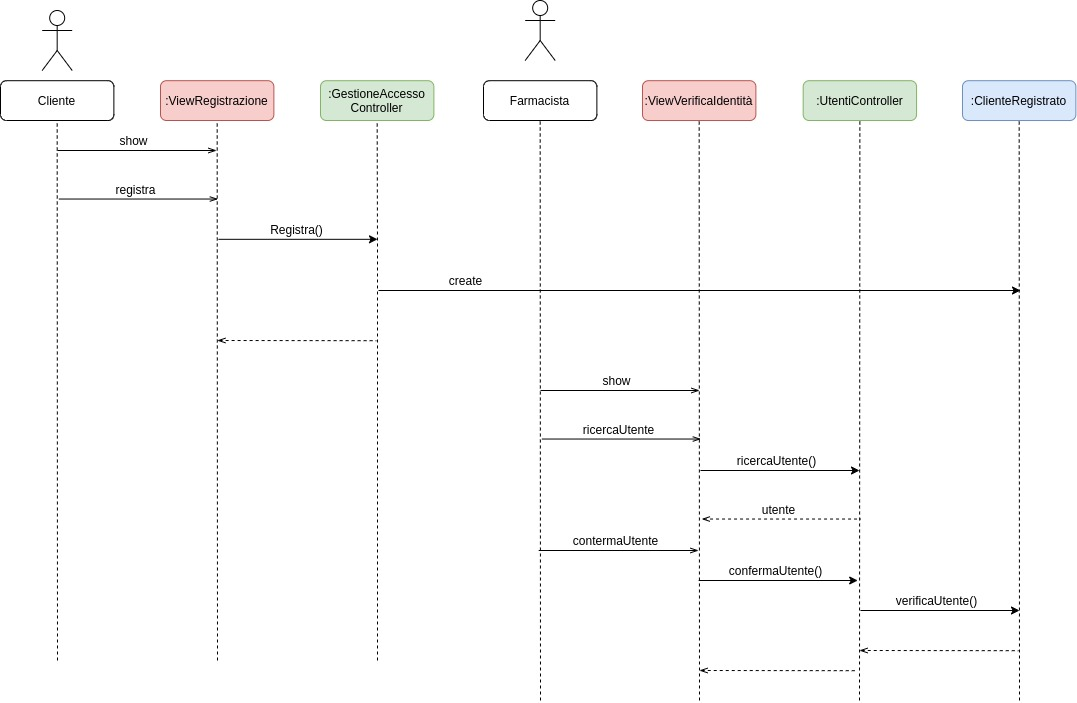
\includegraphics[width=\textwidth]{immagini/Interazione-RegistrazioneUtente.jpg}
    \end{center}
\end{figure}

\newpage
\textbf{Diagramma di Sequenza: VerificaIdentità}

\begin{figure}[h!]
    \begin{center}
        \includegraphics[width=\textwidth]{immagini/Interazione-VerificaIdentità-progettaz.jpg}
        %\caption{Diagramma di Sequenza: VerificaIdentità}
    \end{center}
\end{figure}

\textbf{Diagramma di Sequenza: SospensioneUtenza}
\begin{figure}[h!]
    \begin{center}
        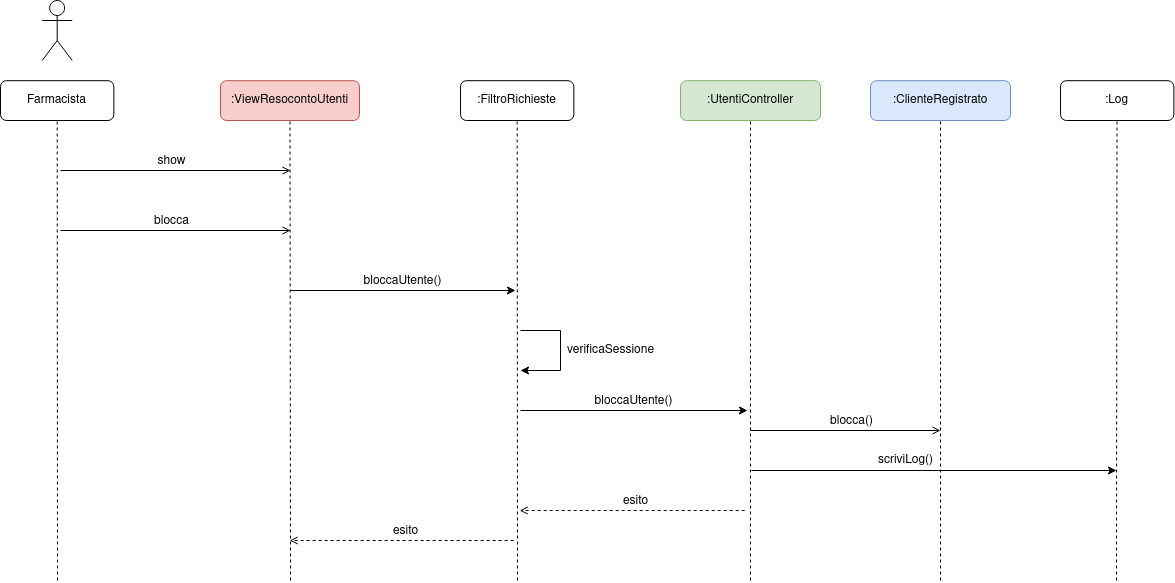
\includegraphics[width=\textwidth]{immagini/Interazione-SospensioneUtenza-progettaz.jpg}
        %\caption{Diagramma di Sequenza: SospensioneUtenza}
    \end{center}
\end{figure}


\newpage

\textbf{Diagramma di Sequenza: NuovaPrenotazione}
\begin{figure}[h!]
    \begin{center}
        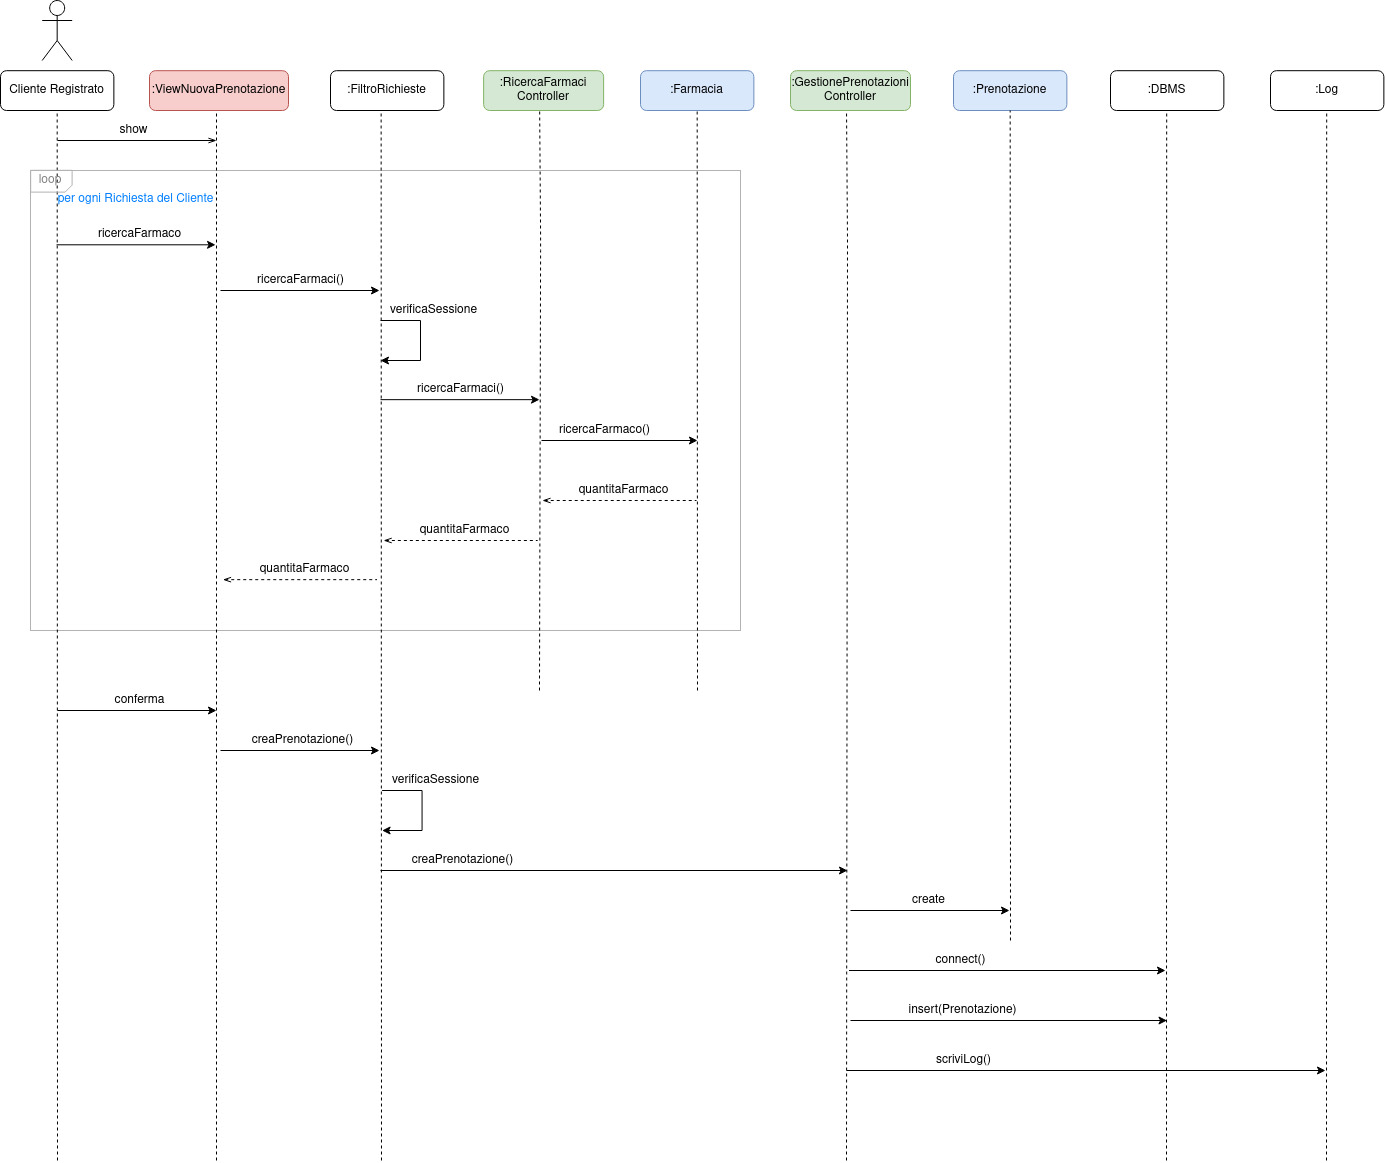
\includegraphics[width=\textwidth]{immagini/Interazione-NuovaPrenotazione-progettaz.jpg}
    \end{center}
\end{figure}

\newpage

\textbf{Diagramma di Sequenza: ConfermaPrenotazione}
\begin{figure}[h!]
    \begin{center}
        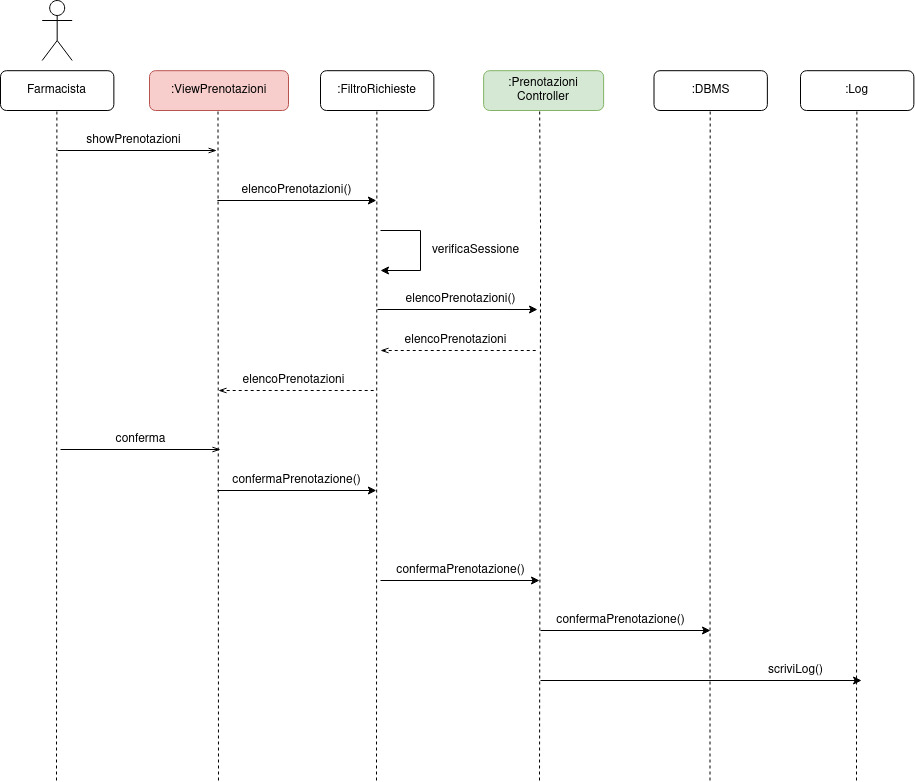
\includegraphics[width=\textwidth]{immagini/Interazione-ConfermaPrenotazione-progettaz.jpg}
    \end{center}
\end{figure}

\newpage

\textbf{Diagramma di Sequenza: RicercaFarmaci}
\begin{figure}[h!]
    \begin{center}
        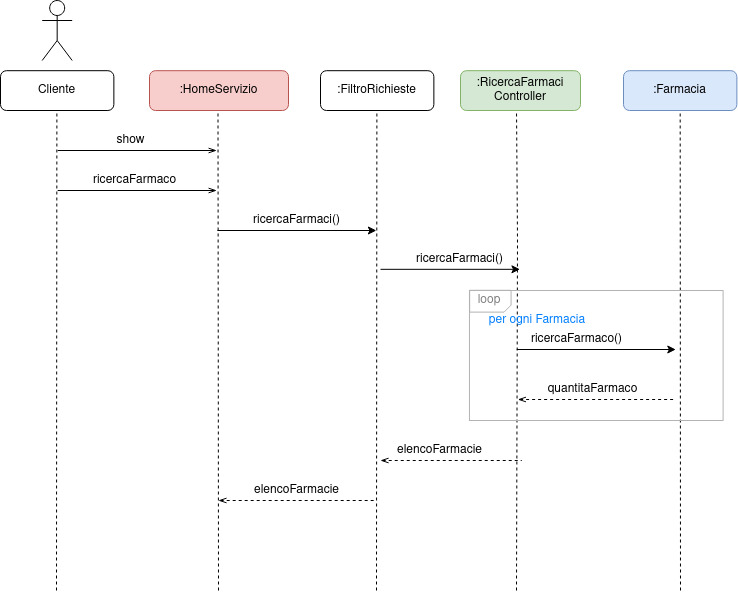
\includegraphics[width=\textwidth]{immagini/Interazione-RicercaFarmaco-progettaz.jpg}
    \end{center}
\end{figure}

\newpage

\subsection{Progettazione della persistenza}

\subsubsection*{Diagramma E-R}

\begin{figure}[h!]
    \begin{center}
        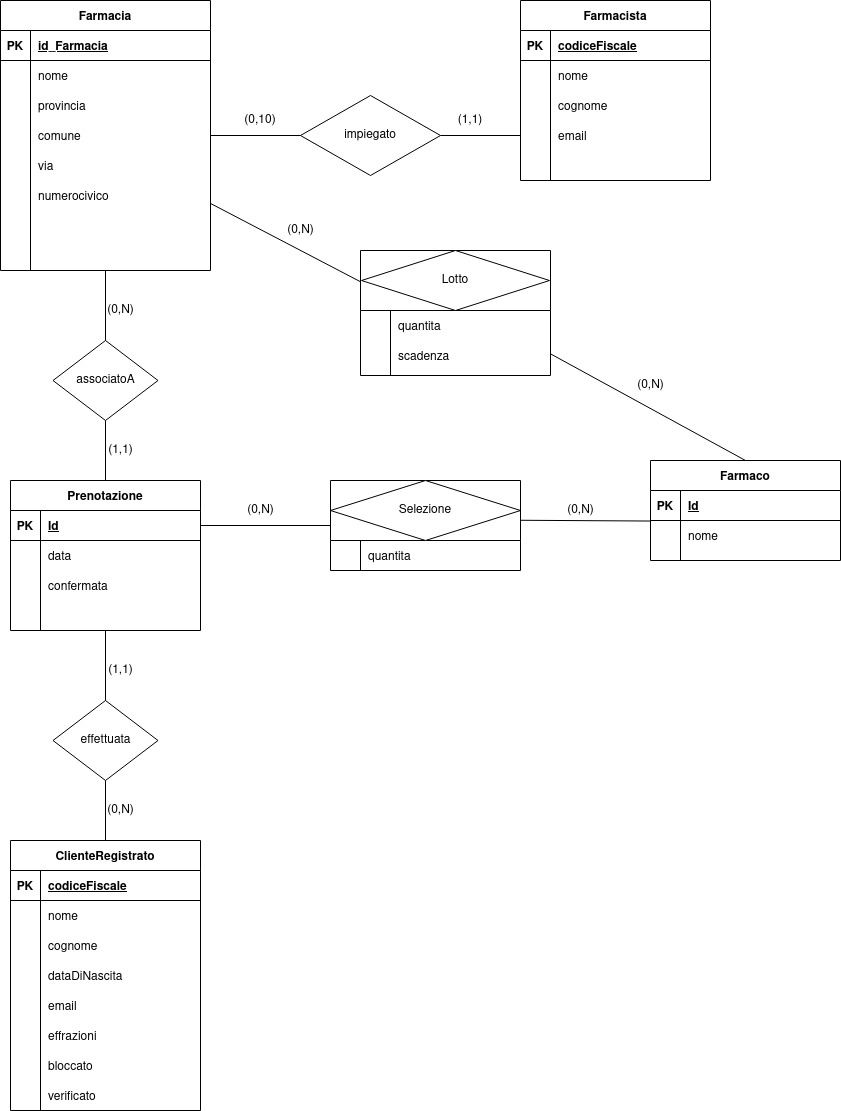
\includegraphics[scale=0.545]{immagini/DiagrammaE-R.jpg}
        %\caption{Persistenza: Diagramma E-R}
    \end{center}
\end{figure}

Come si può notare, il diagramma E-R della persistenza segue precisamente la struttura del modello del dominio mostrato precedentemente.
La differenza sta nelle associazioni, che presumibilmente in fase di progettazione logica ed implementazione del database verranno concretizzate in classi di associazione,
si avranno quindi due tabelle ulteriori (\texttt{Lotto} e \texttt{Selezione}) per modellare le associazioni.

\subsubsection{Formato dei file di log}

Il formato del file di log su cui il sistema terrà traccia delle operazioni
sarà il seguente:\\

Esempio: File \texttt{/var/log/farmabyte.log}\\

\texttt{\$ Data - Ora - Operazione - Descrizione - ID utente}\\
\textbf{Nota}: l'ID utente è l'identificativo dell'esecutore di tale operazione, può essere quindi sia un cliente che un farmacista.
Se nell'eseguire l'operazione, l'utente interagisce o modifica lo stato di altri utenti questo dovrà essere specificato nella descrizione (Caso tipico: farmacista verifica l'identità di un cliente).
L'operazione sarà semplicemente il nome del metodo invocato. 
Si noti infine che ogni riga del file di log inizia con il carattere \texttt{\$}, tale carattere viene usato come delimitatore e non sarà quindi utilizzabile all'interno della descrizione (Né nella definizione degli altri campi).

\newpage

\subsection{Progettazione del collaudo}

Avendo lasciato inalterato il modello del dominio dalla fase di analisi, introducendo solo qualche classe e interfaccia (principalmente per il pattern Observer), 
i test per il collaudo visti in fase di analisi sono stati ritenuti sufficienti.

\vspace{2em}

\subsection{Progettazione per il deployment}

Poiché si è scelto di realizzare il programma come applicazione web, il deployment non necessiterà di particolari configurazioni lato client.
Tutte le interfacce (per clienti, farmacisti, login) sono in realtà memorizzate nel server locale e potranno essere quindi aggiornate automaticamente e in modo centralizzato dagli amministratori di sistema. 

\newpage

\subsection{Deployment}

\subsubsection{Artefatti}

\begin{figure}[h!]
    \begin{center}
        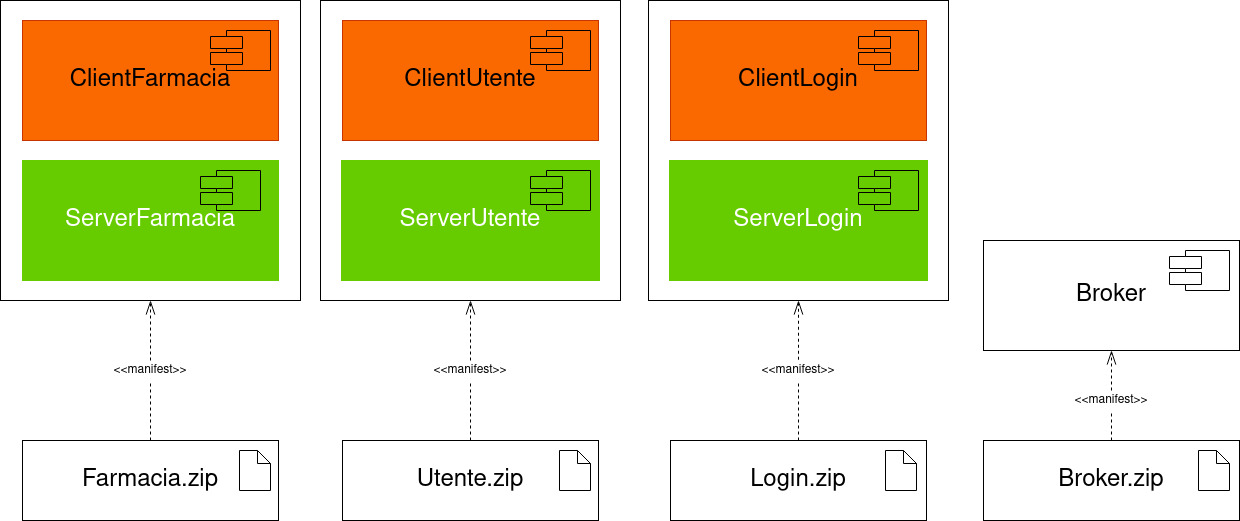
\includegraphics[width=\textwidth]{immagini/Deployment-Artefatti.jpg}
        %\caption{Deployment: Artefatti}
    \end{center}
\end{figure}

\subsubsection{Deployment Type-Level}

\begin{figure}[h!]
    \begin{center}
        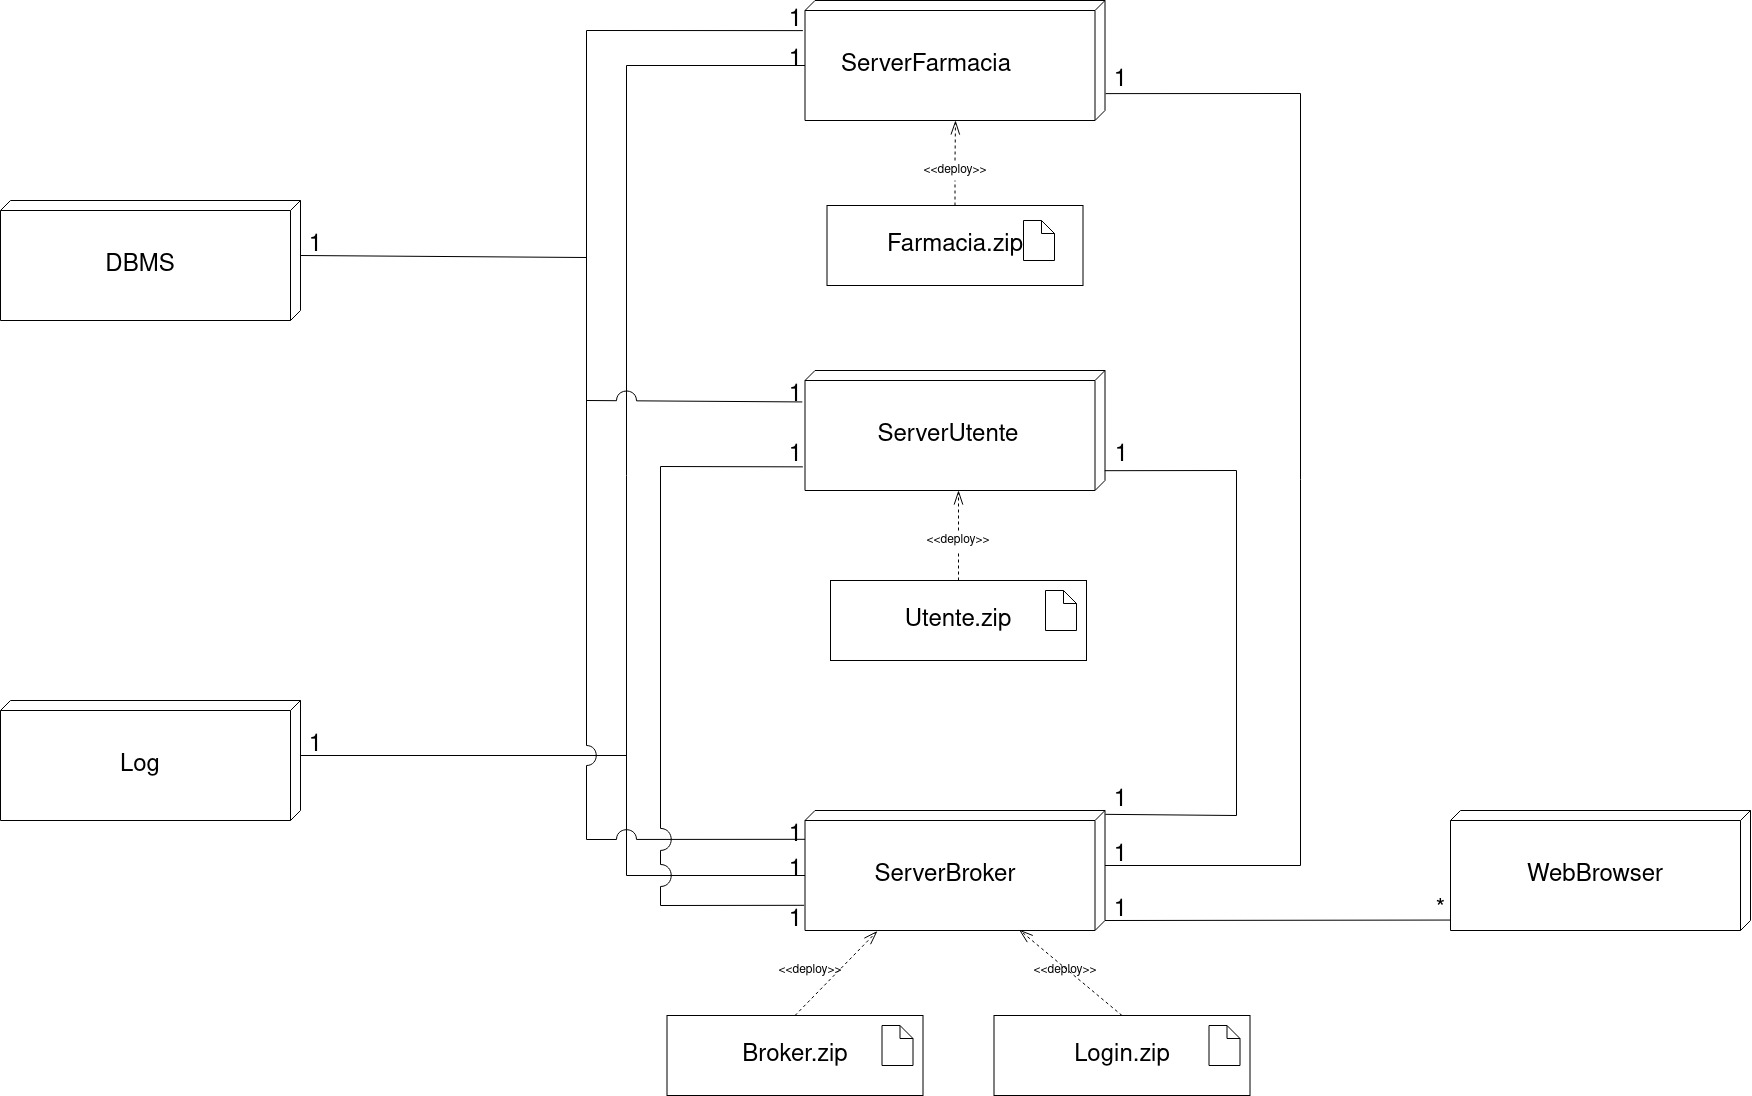
\includegraphics[width=\textwidth]{immagini/Deployment-TypeLevel.jpg}
        %\caption{Deployment Type-Level}
    \end{center}
\end{figure}
